\documentclass{standalone}
\usepackage{tikz}
\begin{document}
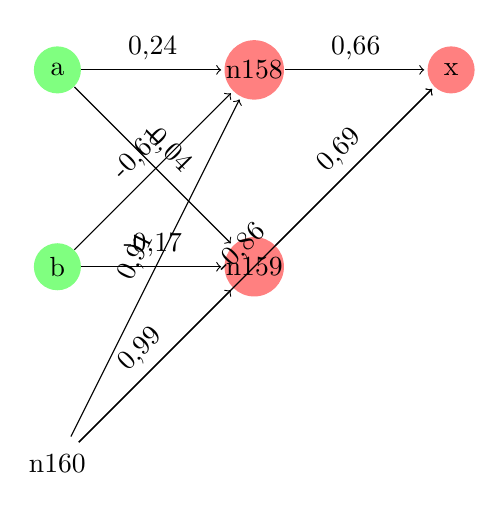
\begin{tikzpicture}[shorten >=1pt,->,draw=black!,node distance=2.5cm]
\tikzstyle{neuron}=[circle,fill=black!25,minimum size=17pt,inner sep=0pt]
\tikzstyle{constant}=[neuron, fill=white!50];
\tikzstyle{sigmoid}=[neuron, fill=red!50];
\tikzstyle{identity}=[neuron, fill=green!50];
\node [identity] (a) {a};
\node [identity,below of=a] (b) {b};
\node [constant,below of=b] (n160) {n160};
\node [sigmoid,right of=a] (n158) {n158};
\node [sigmoid,below of=n158] (n159) {n159};
\node [sigmoid,right of=n158] (x) {x};
\path[every node/.style={sloped,anchor=south,auto=false}]
(n158) edge node {0,66} (x)
(n159) edge node {0,69} (x)
(a) edge node {0,04} (n159)
(a) edge node {0,24} (n158)
(b) edge node {-0,61} (n158)
(b) edge node {-0,17} (n159)
(n160) edge node {0,99} (n159)
(n160) edge node {0,91} (n158)
(n160) edge node {-0,86} (x)
;\end{tikzpicture}
\end{document}